\documentclass[10pt,twoside,a4paper]{article}
\usepackage{pslatex,palatino,avant,graphicx}
\usepackage[usenames,dvipsnames]{color}
\usepackage[margin=2cm]{geometry}
\usepackage{url}
\usepackage[square,sort]{natbib}

\usepackage{listings}
\lstset{ %
  backgroundcolor=\color{white},   % choose the background color; you must add \usepackage{color} or \usepackage{xcolor}
  basicstyle=\footnotesize,        % the size of the fonts that are used for the code
  breakatwhitespace=false,         % sets if automatic breaks should only happen at whitespace
  breaklines=true,                 % sets automatic line breaking
  captionpos=b,                    % sets the caption-position to bottom
  commentstyle=\color{LimeGreen},  % comment style
  % deletekeywords={...},            % if you want to delete keywords from the given language
  escapeinside={\%*}{*)},          % if you want to add LaTeX within your code
  extendedchars=true,              % lets you use non-ASCII characters; for 8-bits encodings only, does not work with UTF-8
  frame=single,                    % adds a frame around the code
  keepspaces=true,                 % keeps spaces in text, useful for keeping indentation of code (possibly needs columns=flexible)
  keywordstyle=\color{BlueGreen},  % keyword style
  % language=Java,                   % the language of the code
  % numbers=left,                    % where to put the line-numbers; possible values are (none, left, right)
  % numbersep=5pt,                   % how far the line-numbers are from the code
  % numberstyle=\tiny\color{Gray},   % the style that is used for the line-numbers
  rulecolor=\color{black},         % if not set, the frame-color may be changed on line-breaks within not-black text (e.g. comments (green here))
  showspaces=false,                % show spaces everywhere adding particular underscores; it overrides 'showstringspaces'
  showstringspaces=false,          % underline spaces within strings only
  showtabs=false,                  % show tabs within strings adding particular underscores
  stepnumber=2,                    % the step between two line-numbers. If it's 1, each line will be numbered
  stringstyle=\color{RubineRed},   % string literal style
  tabsize=2,                       % sets default tabsize to 2 spaces
  title=\lstname,                  % show the filename of files included with \lstinputlisting; also try caption instead of title
  aboveskip=1em,
  belowcaptionskip=0em,
  belowskip=0em
}

\usepackage{hyperref}
\hypersetup{
    colorlinks,
    citecolor=Violet,
    filecolor=black,
    linkcolor=MidnightBlue,
    urlcolor=MidnightBlue
}

\begin{document}
\providecommand{\versionnumber}{0.1.10}
\title{jModelTest 2 Manual v\versionnumber}
\author{Diego Darriba, David Posada}
\date{\today}
\maketitle

\setcounter{tocdepth}{2}
\tableofcontents

\clearpage

\section{Overview}

jModelTest is a tool to carry out statistical selection of best-fit models of nucleotide substitution. It implements five different model selection strategies: hierarchical and dynamical likelihood ratio tests (hLRT and dLRT), Akaike and Bayesian information criteria (AIC and BIC), and a decision theory method (DT). It also provides estimates of model selection uncertainty, parameter importances and model-averaged parameter estimates, including model-averaged tree topologies. jModelTest 2 includes High Performance Computing (HPC) capabilities and additional features like new strategies for tree optimization, model-averaged phylogenetic trees (both topology and branch lenght), heuristic filtering and automatic logging of user activity.

\subsection{Download}

The main project webpage is located at GitHub: \url{https://github.com/ddarriba/jmodeltest2}.

New distributions of jModelTest will be hosted in GitHub releases and google drive.
\begin{itemize}
  \item \url{https://github.com/ddarriba/jmodeltest2/releases}
  \item \url{https://drive.google.com/folderview?id=0ByrkKOPtF_n_OUs3d0dNcnJPYXM#list}
\end{itemize}

Please use the jModelTest discussion group for any question: 
\begin{itemize}
  \item \url{http://groups.google.com/group/jmodeltest}.
\end{itemize}

\subsection{Citation}

When using jModelTest you should cite all these:

\begin{itemize}
\item Darriba D, Taboada GL, Doallo R, Posada D. 2012. jModelTest 2: more models, new heuristics and parallel computing. Nature Methods 9(8), 772.
\item Guindon S and Gascuel O (2003). A simple, fast and accurate method to estimate large phylogenies by maximum-likelihood". Systematic Biology 52: 696-704. 
\end{itemize}

\subsection{Disclaimer}

{\footnotesize
This program is free software; you can redistribute it and/or modify it under the terms of the GNU General Public License as published by the Free Software Foundation; either version 3 of the License, or (at your option) any later version. This program is distributed in the hope that it will be useful, but WITHOUT ANY WARRANTY; without even the implied warranty of MERCHANTABILITY or FITNESS FOR A PARTICULAR PURPOSE. See the GNU General Public License for more details. You should have received a copy of the GNU General Public License along with this program; if not, write to the Free Software Foundation, Inc., 59 Temple Place - Suite 330, Boston, MA 02111-1307, USA. The jModelTest distribution includes Phyml executables.

These programs are protected by their own license and conditions, and using jModelTest implies agreeing with those conditions as well. 
}

%%%%%%%%%%%%%%%%%%%%%%%%%%%%%%%%%%%%%%

{\footnotesize
\subsection{Last Updates}

\begin{itemize}

  \item 3 Mar 2016 Version 2.1.10 Revision 20160303
  \begin{itemize}
    \item Fixed bug with sequences where the 8-char name prefixes are equal
    \item Added warning when the logging is disabled on runtime
    \item Added win32 PhyML binary version to compatibility list
  \end{itemize}

  \item 15 Jan 2016 - Version 2.1.9
  \begin{itemize}
    \item Added automatic search for PhyML binary in /usr/bin
    \item Removed non-ASCII characters
    \item Disable logging if writing is not possible
    \item Merge GUI images into jarfile
  \end{itemize}

  \item 20 Oct 2015 - Version 2.1.8
  \begin{itemize}
    \item Removed ReadSeq dependency
    \item Fixed warnings
    \item Updated prottest jarfile to v3.4
  \end{itemize}


	\item 20 Feb 2015 - Version 2.1.7
	\begin{itemize}
  		\item Fixed bug in ML tree search operation. Console version was using NNI moves instead of "BEST" by default.
	\end{itemize}

	\item 20 Nov 2014 - Version 2.1.7
	\begin{itemize}
		\item Fixed bug with special characters in paths
		\item Added initial check of PhyML binaries
		\item Added notification in case AICc produces negative values
	\end{itemize}

	\item 06 Aug 2014 - Version 2.1.6
	\begin{itemize}
		\item Added confirmation window when cancelling running jobs in the GUI
		\item Added automatic checkpointing files generation
		\item Added ``-ckp'' argument for loading checkpointing files
	\end{itemize}

	\item 05 Apr 2014 - Version 2.1.5
	\begin{itemize}
		\item Updated OS X binary
		\item Fixed bug with computation of JC model for ``fixed'' topology
		\item Fixed bug with DT criterion computation
		\item Added ``-n'' argument for naming executions (the name is included in the log filenames)
		\item Added ``-getphylip'' argument for converting alignments into PHYLIP format with ALTER
		\item Fixed bug in PhyML logging in GUI. Added a unique ID for every model in the log file
		\item Added PAUP* block into log files if required (``-w'' argument)
		\item Added more verbose error messages 
	\end{itemize}

	\item 10 Jul 2013 - Version 2.1.4
	\begin{itemize}
		\item Added phyml auto-logging.
		\item Added phyml command lines for best-fit models.
		\item Added phyml log tab in the GUI.
		\item Removed sample size modes (and ``-n'' argument). Sample size is fixed to alignment size.
		\item Fixed bug with relative paths when calling from a different path.
		\item Fixed typos in the GUI. 
	\end{itemize}

	\item 05 Mar 2013 - Version 2.1.3
	\begin{itemize}
		\item Fixed bug with PAUP`*` command block.
		\item Added the possibility to change Inforation Criterion used with the clustering algorithm for the 203 matrices.
		\item Changed ``-o'' argument for the hypothesis order into ``-O''
		\item Added ``-o'' argument for forwarding the standard output to a file: -o FILENAME 
	\end{itemize}

	\item 01 Jan 2013 Version 2.1.2 - Revision 20130103
	\begin{itemize}
		\item Fixed bug in paths with whitespaces.
		\item Updated PhyML binaries. 
	\end{itemize}

	\item 31 Jul 2012 Version 2.1.1 - Revision 20120731
	\begin{itemize}
		\item Fixed bug with hLRT selection when attempting to use a user-defined topology. 
	\end{itemize}

	\item 11 Mar 2012 Version 2.1 - Revision 20120511
	\begin{itemize}
		\item Major updates:
		\begin{itemize}
			\item Exhaustive GTR submodels: All the 203 different partitions of the GTR rate matrix can be included in the candidate set of models. When combined with rate variation (+I,+G, +I+G) and equal/unequal base frequencies the total number of possible models is 203 x 8 = 1624. 
			\item Hill climbing hierarchical clustering: Calculating the likelihood score for a large number of models can be extremely time-consuming. This hill-climbing algorithm implements a hierarchical clustering to search for the best-fit models within the full set of 1624 models, but optimizing at most 288 models while maintaining model selection accuracy. 
			\item Heuristic filtering: Heuristic reduction of the candidate models set based on a similarity filtering threshold among the GTR rates and the estimates of among-site rate variation. 
			\item Absolute model fit: Information criterion distances can be calculated for the best-fit model against the unconstrained multinomial model (based on site pattern frequencies). This is computed by default when the alignment does not contain missing data/ambiguities, but can also be approximated otherwise. 
			\item Topological summary: Tree topologies supported by the different candidate models are summarized in the html log, including confidence intervals constructed from cumulative models weights, plus Robinson-Foulds and Euclidean distances to the best-fit tree for each. 
		\end{itemize}
		\item Minor updates:
		\begin{itemize}
			\item Corrected a bug in the fixed BIONJ-JC starting topology. F81+I+G was executed instead of JC.
			\item ``Best'' is now the default tree search operation instead of NNI. ``Best'' computes both NNI and SPR algorithms and selects the best of them.
			\item User can select the number of threads from GUI. 
		\end{itemize}
	\end{itemize}


	\item 1 Feb 2012 - Version 2.0.2

	\begin{itemize}
		\item Added a selection summary at the end of the console output.
		\item Corrected the table header in the DT results frame (sorting).
		\item Corrected a bug in DT Criterion where selection could not take place with large alignments.
		\item Corrected a bug with command console version, where the execution crashed with certain arguments.
		\item Unified LOCALE for English format. 
	\end{itemize}

	\item 2 Nov 2011 - Version 2.0.1

	\begin{itemize}
		\item Improved thread scheduling algorithm.
		\item OpenMP phyml patch for hybrid execution.
		\item New argument (machinesfile) for hybrid execution on heterogeneous architectures, or heterogeneous resources distribution. 
	\end{itemize}

	\item 13 Oct 2011 - Revision 20111013

	\begin{itemize}
		\item Added conf/jmodeltest.conf file, where you can:
			Enable/Disable the automatic logging:

			    You might be running a huge dataset and you don't want to generate hundreds or thousands of log files. 

			Set the PhyML binaries location:

			    If you already have installed PhyML in your machine, you can setup jModelTest for use your own binaries. 

		\item Enhanced the html log output. 
	\end{itemize}

\end{itemize}


}

%%%%%%%%%%%%%%%%%%%%%%%%%%%%%%%%%%%%%%

\section{Getting Started}

\subsection{Operating Systems}

Since jModelTest is a Java application, it can be used in every OS that can execute a Java Runtime Environment (JRE). The most common Operating Systems and many other include a JRE (OpenJDK, Sun JRE, ...), or at least it is possible to download one. However, jModelTest depends on third-party binaries (PhyML), that are distributed for Windows, Linux and OsX, and it is even possible to download PhyML sources (http://code.google.com/p/phyml) and compile them for a particular architecture.

\subsection{Working with the repository}

This tool is distributed under GPL v3 license. The source code is freely available at google code repository. You can checkout the repository at \url{http://code.google.com/p/jmodeltest2/source}.

\subsection{User interfaces}

jModelTest can be executed from two different user interfaces, GUI or Console. The Graphical User Interface (GUI) is intended for execution on common desktop computers with multicore processors -most users will probably use this. On the other hand, HPC environments, like multicore clusters, require a non-interactive processing (batch processes), so jModelTest has to be executed from the Command Console Interface. Results are given in plain text format, but an html log is also created.

\subsubsection{Graphical User Interface}

\begin{enumerate}
\item Execute the script for the Graphical User Interface (runjmodeltest-gui.sh). The main jModelTest frame should pop up on the screen:

\begin{center}
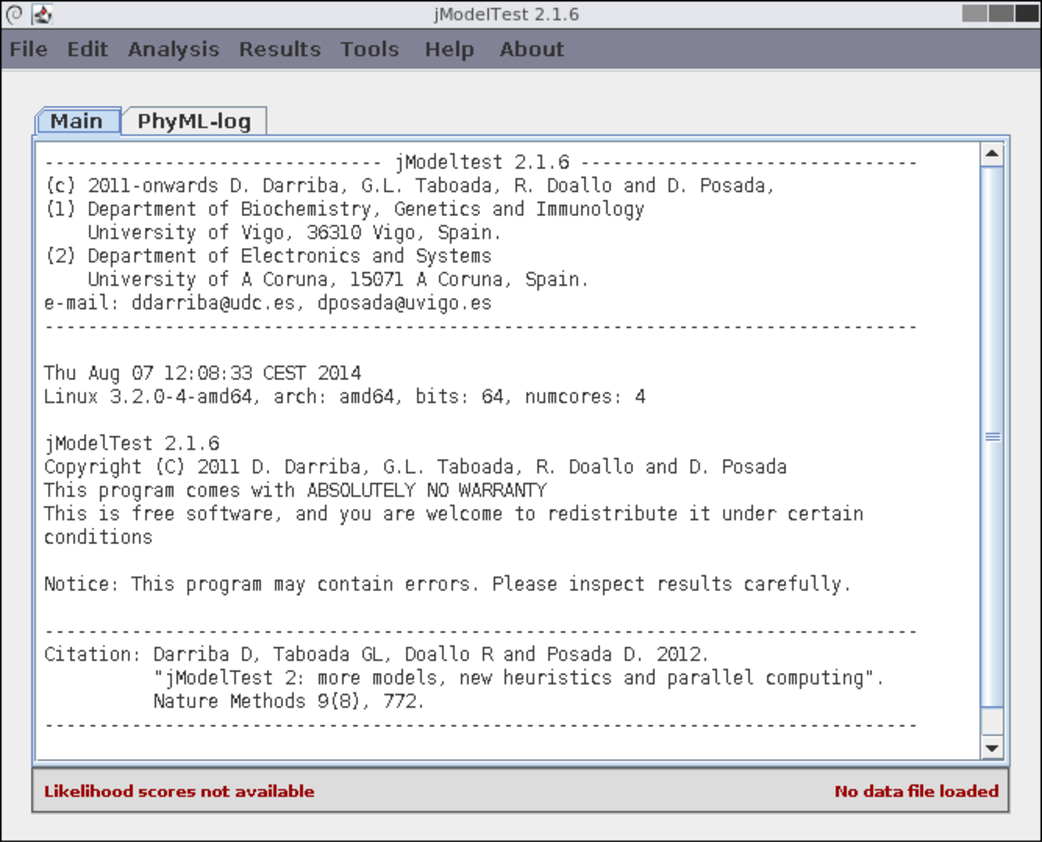
\includegraphics[width=.9\textwidth]{images/main-window.pdf}
\end{center}

\item Load an input alignment file using the {\bf File/Load Alignment} option.

\item Go to {\bf Analysis/Compute Likelihood Scores} and select the candidate models and the options for model optimization (optionally you can set a base topology from a file). Press Enter or the {\bf Compute Likelihoods} button.

\begin{center}
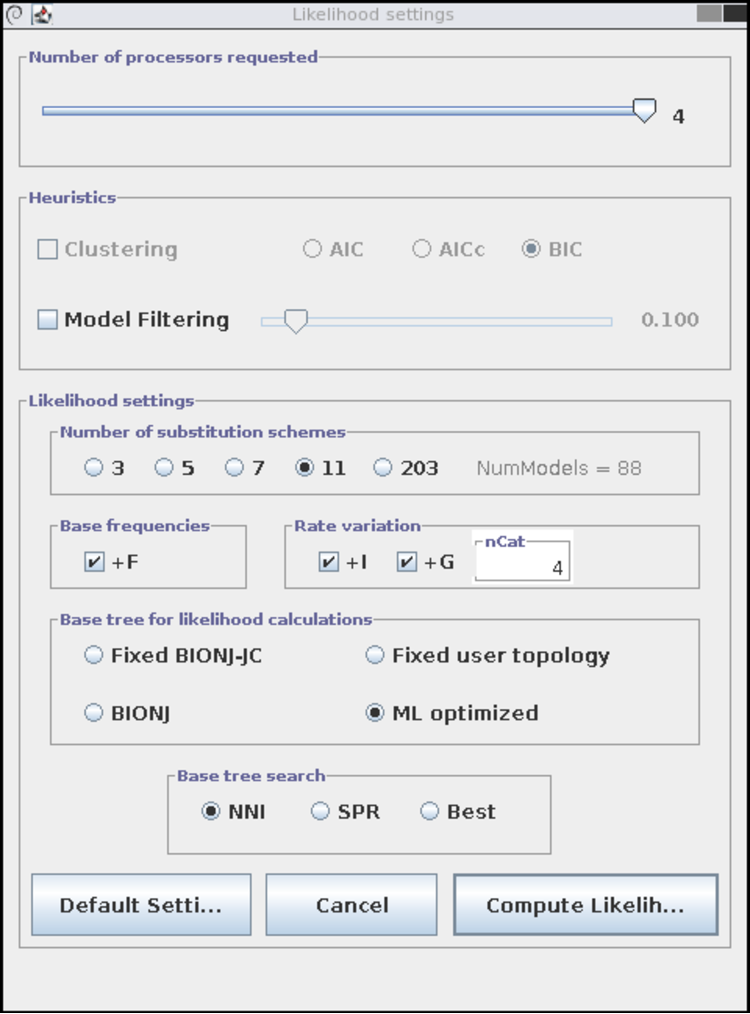
\includegraphics[width=.6\textwidth]{images/lkl-settings.pdf}
\end{center}

\item Perform statistical selection among the optimized models. For example, we can calculate the Bayesian Information Criterion using {\bf Analysis/Do BIC calculations...} option, or any other. You can find a Criteria comparison in terms of accuracy in the \href{http://www.nature.com/nmeth/journal/v9/n8/extref/nmeth.2109-S1.pdf}{supplementary material} of the \href{http://www.nature.com/nmeth/journal/v9/n8/full/nmeth.2109.html}{jModelTest publication}.

\begin{center}
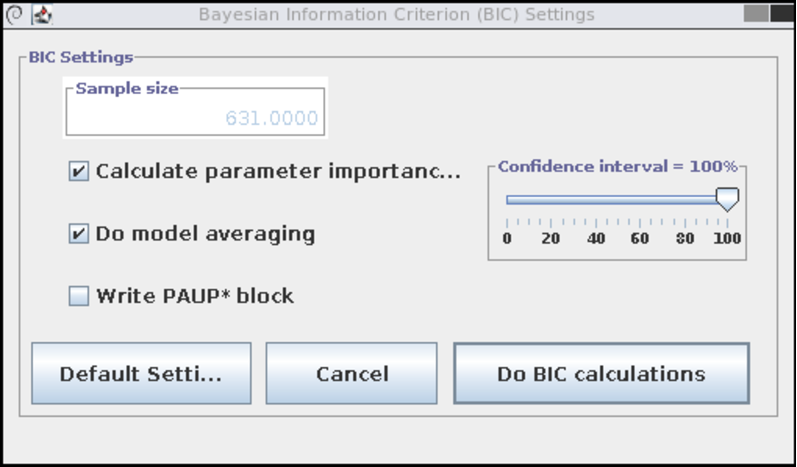
\includegraphics[width=.6\textwidth]{images/bic.pdf}
\end{center}

The results will be shown in the main console.

\item Take a look at the results table in {\bf Results/Show results table}. Best model is the one with the lowest criterion value (BIC column in the example) and therefore delta = 0.

\begin{center}
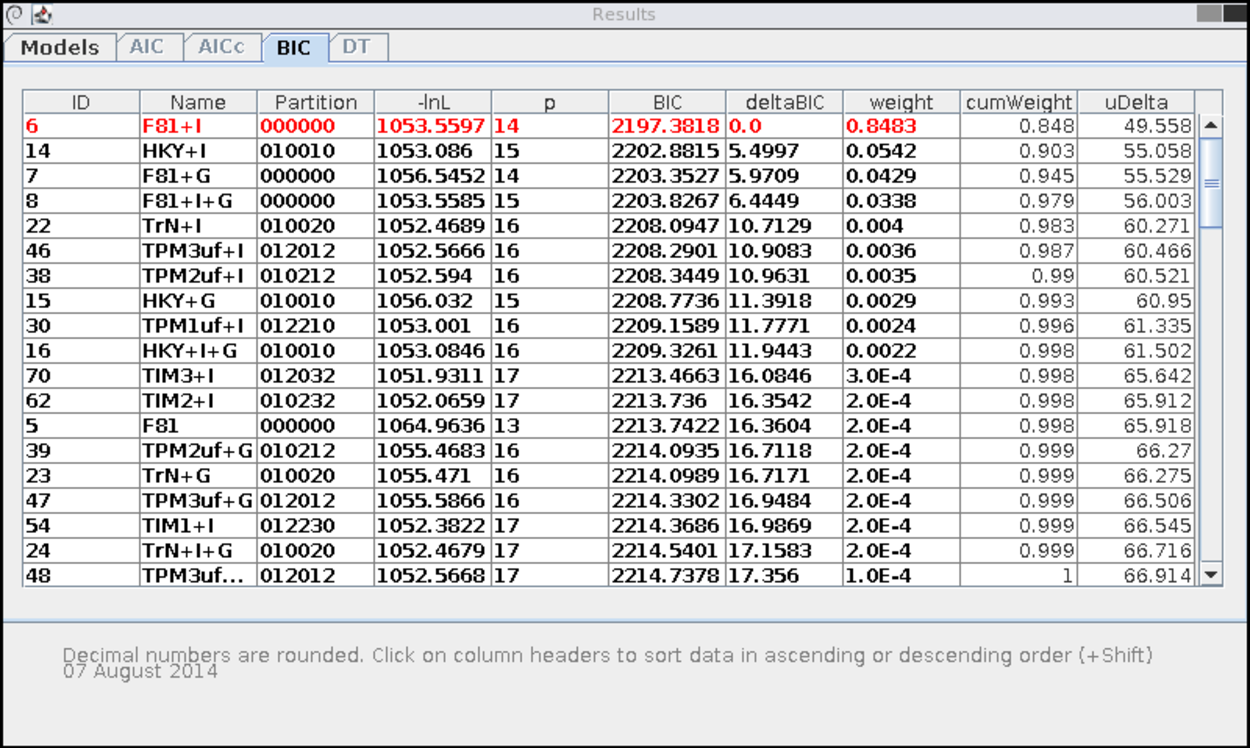
\includegraphics[width=.9\textwidth]{images/results.pdf}
\end{center}

\item Build a consensus tree from a given selection criteria using {\bf Analysis/Model-averaged phylogeny}:

\begin{center}
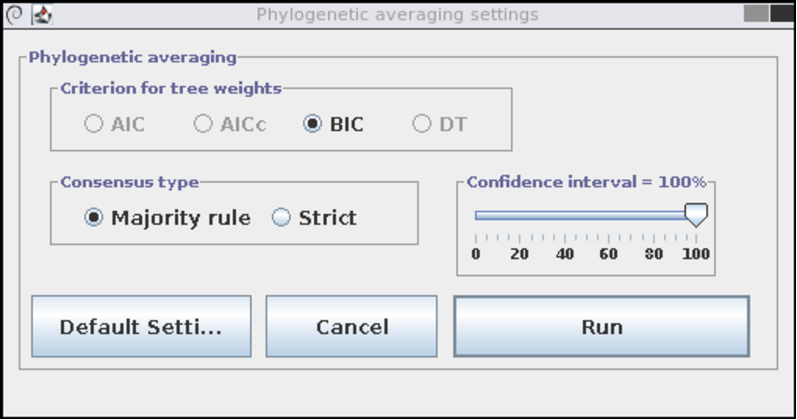
\includegraphics[width=.6\textwidth]{images/consensus.pdf}
\end{center}

\item Finally, you can save the results displayed in the main console using {\bf Edit/Save console}. Alternatively, you can get a formatted HTML document using {\bf Results/Build HTML log}:

\begin{center}
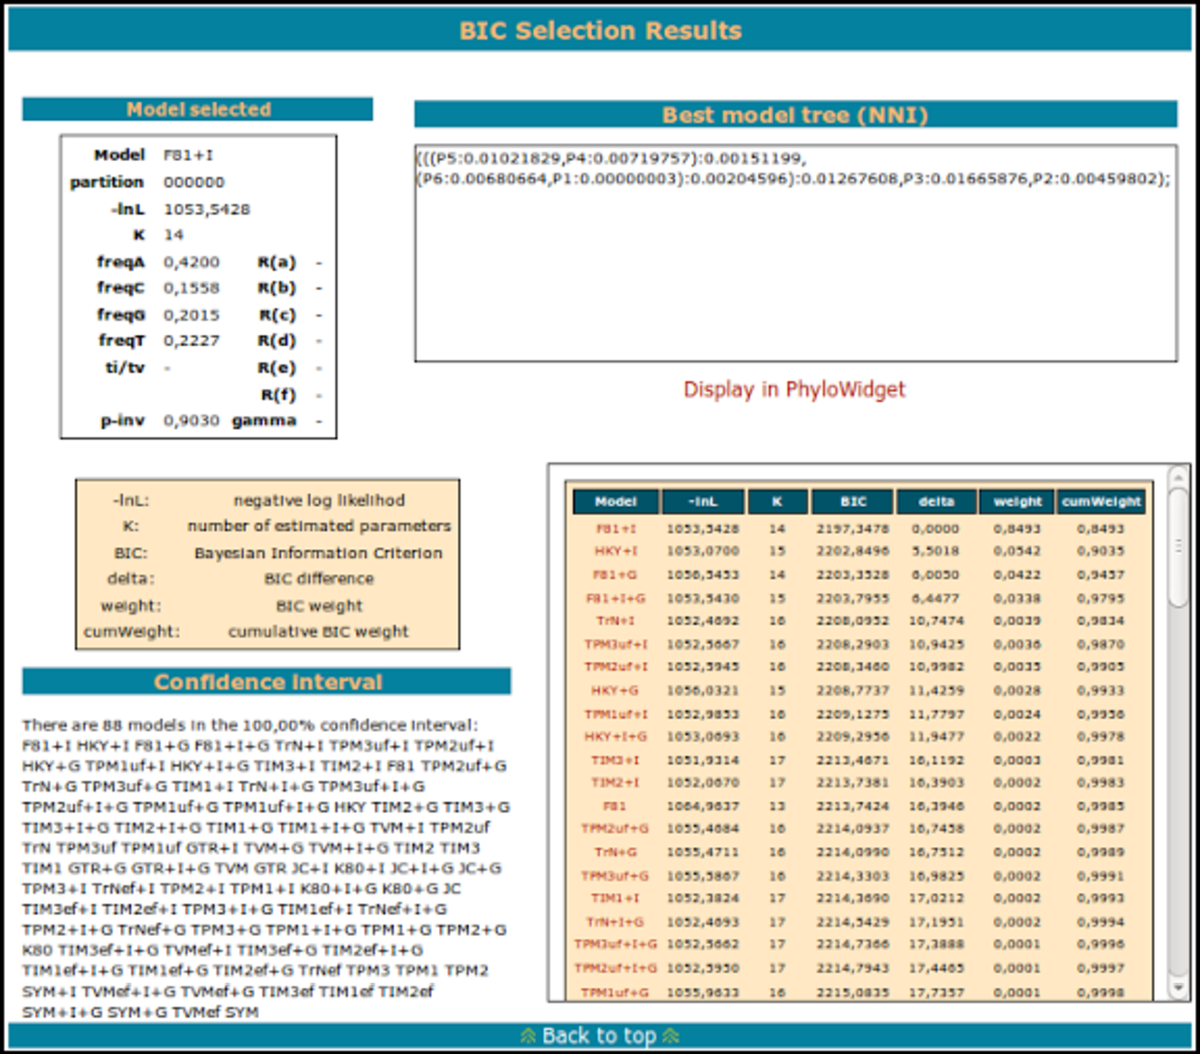
\includegraphics[width=.9\textwidth]{images/html-log.pdf}
\end{center}

Take a look at Section \ref{sec:gui} for further information.

\end{enumerate}

\subsubsection{Command Console Interface}

\begin{enumerate}
\item Execute the following command line:
\begin{lstlisting}
$ java -jar jModelTest.jar -d example-data/aP6.fas -g 4 -i -f -AIC -BIC -a
\end{lstlisting}

This will test all 88 models (gamma models with 4 rate categories), and then perform the model selection using Akaike (AIC) and Bayesian (BIC) criteria, calculating also a model averaged phylogeny (-a).

See Section~\ref{sec:arguments} for information about supported arguments.

\item This will generate the following output:

\begin{enumerate}

\item Header:

\begin{lstlisting}
----------------------------- jModeltest 2.0 -----------------------------
(c) 2011-onwards Diego Darriba, David Posada,
Department of Biochemistry, Genetics and Immunology
University of Vigo, 36310 Vigo, Spain. e-mail: ddarriba@udc.es, dposada@uvigo.es
--------------------------------------------------------------------------------
Wed Oct 05 12:56:47 CEST 2011
Linux 2.6.38-11-generic-pae, arch: i386, bits: 32, numcores: 2

jModelTest 2.0  Copyright (C) 2011 Diego Darriba, David Posada
This program comes with ABSOLUTELY NO WARRANTY
This is free software, and you are welcome to redistribute it
under certain conditions
 
Notice: This program may contain errors. Please inspect results carefully.
\end{lstlisting}

\item Execution options:

\begin{lstlisting} 
Arguments = -d example-data/aP6.fas -g 4 -i -f -AIC -BIC -a

Reading data file "aP6.fas"... OK.
  number of sequences: 6
  number of sites: 631
 
 
---------------------------------------------------------------
*                                                             *
*        COMPUTATION OF LIKELIHOOD SCORES WITH PHYML          *
*                                                             *
---------------------------------------------------------------
 
::Settings::
 Phyml version = 3.0
 Phyml binary = PhyML_3.0_linux32
 Candidate models = 24
  number of substitution schemes = 3
  including models with equal/unequal base frequencies (+F)
  including models with/without a proportion of invariable sites (+I)
  including models with/without rate variation among sites (+G) (nCat = 4)
 Optimized free parameters (K) = substitution parameters + 9 branch lengths + topology 
 Base tree for likelihood calculations = ML tree
 Tree topology search operation = NNI
computing likelihood scores for 24 models with Phyml 3.0
\end{lstlisting}

\item Real time optimization results (progress):

\begin{lstlisting}
::Progress::

Model 		 Exec. Time 	 Total Time 	 -lnL
-------------------------------------------------------------------------
JC		00h:00:00:01	00h:00:00:01	1114,9772
JC+G		00h:00:00:04	00h:00:00:05	1106,4431
...
GTR+G		00h:00:00:06	00h:00:06:07	1054,7203
GTR+I+G		00h:00:01:02	00h:00:07:05	1051,8403
\end{lstlisting}

\item Sorted and complete optimization results:

\begin{lstlisting}
   Model = JC
   partition = 000000
   -lnL = 1114.9772
   K = 10 
 
   Model = JC+I
   partition = 000000
   -lnL = 1103.1113
   K = 11
   p-inv = 0.9080 

...

   Model = GTR+I+G
   partition = 012345
   -lnL = 1051.8403
   K = 20
   freqA = 0.4235 
   freqC = 0.1520 
   freqG = 0.2022 
   freqT = 0.2224 
   R(a) [AC] =  0.8709
   R(b) [AG] =  0.4152
   R(c) [AT] =  0.6049
   R(d) [CG] =  1.2523
   R(e) [CT] =  0.9482
   R(f) [GT] =  1.0000
   p-inv = 0.5940
   gamma shape = 0.0120 
 
 
Computation of likelihood scores completed. It took 00h:00:07:05.
\end{lstlisting}

\item Selected Information Criteria (best model and all models sorted according to each criterion):

\begin{lstlisting}
---------------------------------------------------------------
*                                                             *
*             AKAIKE INFORMATION CRITERION (AIC)              *
*                                                             *
---------------------------------------------------------------
 
 Model selected: 
   Model = F81+I
   partition = 000000
   -lnL = 1053.5428
   K = 14
   freqA = 0.4200 
   freqC = 0.1558 
   freqG = 0.2015 
   freqT = 0.2227 
   p-inv = 0.9030 
 
ML tree (NNI) for the best AIC model = (((P5:0.01021829,P4:0.00719757):0.00151199,(P6:0.00680664,P1:0.00000003):0.00204596):0.01267608,P3:0.01665876,P2:0.00459802);
 
 
* AIC MODEL SELECTION : Selection uncertainty
 
Model             -lnL    K         AIC      delta      weight cumWeight
------------------------------------------------------------------------ 
F81+I        1053.5428   14   2135.0855     0.0000      0.4332    0.4332 
HKY+I        1053.0700   15   2136.1401     1.0545      0.2557    0.6890 
F81+I+G      1053.5430   15   2137.0859     2.0004      0.1594    0.8483
...
K80          1114.5049   11   2251.0098   115.9243   2.91e-026    1.0000 
SYM          1114.4117   15   2258.8235   123.7380   5.85e-028    1.0000
------------------------------------------------------------------------
-lnL:	negative log likelihod
 K:	number of estimated parameters
 AIC:	Akaike Information Criterion
 delta:	AIC difference
 weight:	AIC weight
 cumWeight:	cumulative AIC weight
 
 
* AIC MODEL SELECTION : Confidence interval
 
There are 24 models in the 100% confidence interval: [ F81+I HKY+I F81+I+G HKY+I+G F81+G GTR+I HKY+G GTR+I+G GTR+G F81 HKY GTR JC+I K80+I JC+I+G K80+I+G JC+G K80+G SYM+I SYM+I+G SYM+G JC K80 SYM ] 
\end{lstlisting}

\item Consensus tree of the optimized phylogenies using the criterion weights:
 
\begin{lstlisting}
---------------------------------------------------------------
*                                                             *
*                    MODEL AVERAGED PHYLOGENY                 *
*                                                             *
---------------------------------------------------------------
 
Selection criterion: . . . . AIC
Confidence interval: . . . . 1.00
Consensus type:. . . . . . . 50% majority rule
 
 
Using 24 models in the 1.00 confidence interval = F81+I HKY+I F81+I+G HKY+I+G F81+G GTR+I HKY+G GTR+I+G GTR+G F81 HKY GTR JC+I K80+I JC+I+G K80+I+G JC+G K80+G SYM+I SYM+I+G SYM+G JC K80 SYM  

Bipartitions included in the consensus tree
 
    123456
    ****** ( 1.0 )
    ****-- ( 1.0 )
    **---- ( 0.94244 )
    --**-- ( 1.0 )

 
                        +-----------6 P4
                      +-8
                      | +----------------5 P5
+---------------------9
|                     |  +-4 P1
|                     +--7
|                        +----------3 P6
|
+------2 P2
|
+---------------------------1 P3

 
(P3:0.016613,P2:0.004598,((P6:0.006790,P1:0.000000)1.00:0.002046,(P5:0.010191,P4:0.007198)0.94:0.001510)1.00:0.012665);
 
Note: this tree is unrooted. Branch lengths are the expected number of substitutions per site. Labels next to parentheses represent phylogenetic uncertainty due to model selection (see documentation)
\end{lstlisting}

\item Also a HTML log is automatically stored in the ``log'' directory.

\end{enumerate}
\end{enumerate}

\subsection{High Performance Environments}

\subsubsection{Shared memory architectures (multicore systems)}

Both the GUI and Console interfaces can be used for shared memory architectures. See Graphical User Interface or Command Console Interface. In some dedicated HPC environments you can only use the console interface, for example when using a bath-queuing system like Oracle Grid Engine. Additionally, in the console version you can specify the number of threads you want to use using the -tr'' option. By default, the total number of cores in the machine is used.

\subsubsection{Distributed memory architectures (HPC clusters)}

\begin{enumerate}
\item Besides the multithreading support, it is possible to run jModelTest in a cluster. This feature has been implemented using a Java message-passing (MPJ) library, MPJ Express (http://mpj-express.org/). To execute jModelTest in a cluster environment you have to:

\begin{lstlisting}
$ export $JMODELTEST_HOME=[path_to_jModelTest]
$ cd $JMODELTEST_HOME
$ tar zvxf mpj.tar.gz
$ export MPJ_HOME=$JMODELTEST_HOME/mpj
$ export PATH=$MPJ_HOME/bin:$PATH
$ cp $JMODELTEST_HOME/extra/machines $JMODELTEST_HOME
\end{lstlisting}

You can also add the last two lines to ~/.bashrc to automatically set these variables at console startup.

\item \$JMODELTEST\_HOME/machines file contains the set of computing nodes where the mpj processes will be executed. By default it points to the localhost machine, so you should change it if you want to run a parallel execution over a cluster machine, just writing on each line the particular computing nodes (e.g. see filecluster8.conf.template).

\item Start the MPJ Express daemons:

\begin{lstlisting}
$ mpjboot machines
\end{lstlisting}

The application ``mpjboot'' should be in the execution path (it is located at \$MPJ\_HOME/bin). A ssh service must be running in the machines listed in the machines file. Moreover, port 10000 should be free. For more details refer to the MPJ Express documentation.

\item Run jModelTest. For this, the jModelTest distribution provides a bash script: 'runjmodeltest-cluster.sh'

The basic syntax is:

./runjmodeltest-cluster.sh \$NUMBER\_OF\_PROCESSORS \$APPLICATION\_PARAMETERS

\begin{lstlisting}
$ ./runjmodeltest-cluster.sh 2 -d example-data/aP6.fas -s 11 -i -g 4 -f -AIC -a
\end{lstlisting}

\end{enumerate}


%%%%%%%%%%%%%%%%%%%%%%%%%%%%%%%%%%%%%%%%%%%%%%%%%%%%%%%%%%%

\section{Graphical User Interface}
\label{sec:gui}

\subsection{Launching the Graphical User Interface}

The main distribution includes a script for launching the interface,  \emph{runjmodeltest-gui.sh}, located under the jModelTest home folder. Other possibility is running the following command line:

\begin{lstlisting}
$ java -jar jModelTest.jar
\end{lstlisting}

Moreover, in Windows and MacOS X, it is often possible to double-click the jModelTest.jar file to launch the graphical interface.

The following window will show on the screen:

\begin{center}
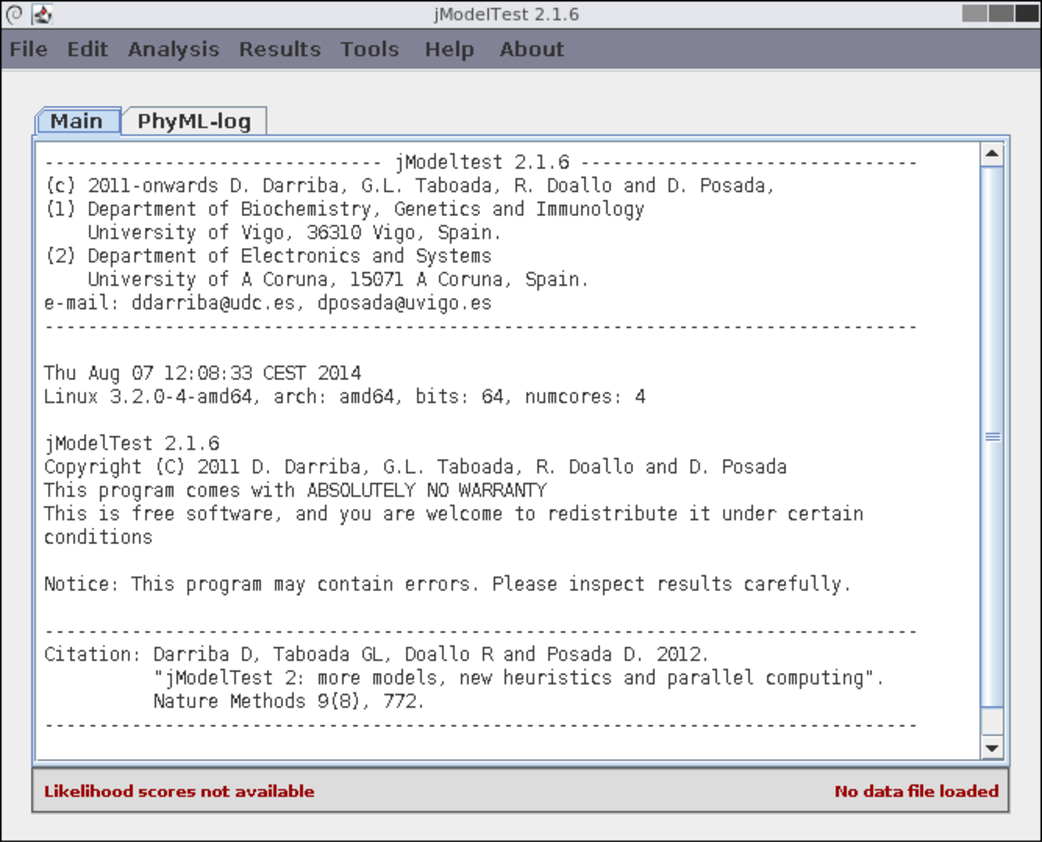
\includegraphics[width=.9\textwidth]{images/main-window}
\end{center}

\subsection{Menu description}

\begin{minipage}{1\textwidth}
\small
\begin{tabular}{l l l l}
\hline
{\bf Menu} & {\bf Submenu} & {\bf Description} & {\bf Enabled} \\
\hline
File \\
& Load alignment & Load an input alignment & \\
& Load checkpoint file & Load a previous snapshot \footnote{See Section~\ref{sec:ckp}} & (i) \\
& Quit & Exit the program & \\
\hline
Analysis \\
& Compute likelihood scores & Optimize the set of candidate models & (i) \\
& Do AIC calculations & Calculate Akaike Information Criterion & (ii) \\
& Do BIC calculations & Calculate Bayesian Information Criterion & (ii) \\
& Do DT calculations & Calculate Decision Theory & (ii) \\
& Do hLRT calculations & Calculate hierarchical likelihood ratio test & (ii) \footnote{This test is only available for 3,5,7 and 11 substitution schemes and for fixed topologies (fixed BIONJ-JC tree or user-defined topology)} \\
& Model-averaged phylogeny & Calculate the consensus tree & (iii \& iv)  \\
\hline
Results \\
& Show results table & Show a table with the selection results & (ii) \\
& Build HTML log & Create an html webpage with the results & (ii) \\
\hline
Tools \\
& LRT calculator & Likelihood Ratio Test for nexted models & \\
\hline
\end{tabular}

\vspace{1em}
(i) After loading an alignment (ii) After computing the likelihood scores (iii) If the base tree is not fixed (iv) After calculating an Information Criterion
\end{minipage}

%%%%%%%%%%%%%%%%%%%%%%%%%%%%%%%%%%%%%%%%%%%%%%%%%%%%%%%%%%%

\section{Command Line Arguments}
\label{sec:arguments}

\begin{itemize}

\item  {\bf -a}

Estimate model-averaged phylogeny for each active criterion. See Section \ref{sec:consensus} for more details.

\item  {\bf -AIC}

Calculate the Akaike Information Criterion. See Section \ref{sec:aic}.

\item  {\bf -AICc}

Calculate the corrected Akaike Information Criterion. See Section \ref{sec:aic}.

\item  {\bf -BIC}

Calculate the Bayesian Information Criterion. See Section \ref{sec:bic}.

\item  {\bf -DT}

Calculate the decision theory criterion. See Section \ref{sec:dt}.

\item  {\bf -c} confidenceInterval

Sets the confidence interval for the model selection process (default is 100).

\item  {\bf -d} inputFile

Sets the input data file. jModelTest makes use of the ALTER library for converting several alignment formats to PHYLIP.

\item  {\bf -dLRT}

Perform dynamical likelihood ratio tests. See Section \ref{sec:dlrt} for more details.

\item  {\bf -f}

Include models with unequals base frecuencies.

\item  {\bf -g} numberOfRateCategories

Include models with rate variation among sites and sets the number of categories. Usually 4 categories are enough.

\item  {\bf -getPhylip}

Converts the input file into phylip format and exits. For example, the following command will generate a new PHYLIP file named ``input.nex.phy''.
\begin{lstlisting}
$java -jar jModelTest.jar -d input.nex -getPhylip
\end{lstlisting}

\item  {\bf -G} threshold

Heuristic search. Requires a threshold > 0 (e.g., -G 0.1)

\item  {\bf -h} confidenceInterval

Sets the confidence level for the hLRTs (default is 0.01)

\item  {\bf -help}

Displays a help message

\item  {\bf -hLRT}

Perform hierarchical likelihood ratio tests. See Section \ref{sec:hlrt} for more details.

\item  {\bf -H}

Information criterion for clustering search (AIC, AICc, BIC). (e.g., -H AIC) (default is BIC)

\item  {\bf -i}

Include models with a proportion invariable sites.

\item  {\bf -machinesfile} machinesFile

Gets the processors per host from a machines file (for MPI execution).

\item  {\bf -n} logSuffix

Execution name appended to the log filenames. By default, current time is used: yyyyMMddhhmmss.

\item  {\bf -o} outputFile

Redirects the output to a file.

\item  {\bf -O} {ftvwxgp}

Sets the hypothesis order for the hLRTs (e.g., -hLRT -O gpftv) (default is ftvwxgp)
\begin{itemize}
\item {\bf f} frequencies
\item {\bf t} transition/transversion ratio
\item {\bf v} 2ti4tv for subst=3 / 2ti for subst>3
\item {\bf w} 2tv
\item {\bf x} 4tv
\item {\bf g} gamma
\item {\bf p} proportion of invariable sites
\end{itemize}

See Section \ref{sec:hlrt} for more details.

\item  {\bf -p}

Calculate the parameter importances. See Section \ref{sec:param-importances}.

\item  {\bf -r}

Backward selection for the hLRT (default is forward).

\item  {\bf -s} 3|5|7|11|203

Sets the number of substitution schemes.
\begin{itemize}
     \item {\bf 3} JC/F81, K80/HKY, SYM/GTR (used by default).
     \item {\bf 5} JC/F81, K80/HKY, TrNef/TrN, TPM1/TPM1uf, SYM/GTR.
     \item {\bf 7} JC/F81, K80/HKY, TrNef/TrN, TPM1/TPM1uf, TIM1ef/TIM1, TVMef/TVM, SYM/GTR.
     \item {\bf 11} All models defined in Table~\ref{table-models}.
     \item {\bf 203} All possible GTR submatrices.
\end{itemize}

\item  {\bf -S} NNI|SPR|BEST

Defines the tree topology search operation option for Maximum-Likelihood search: 
\begin{itemize}
     \item {\bf NNI} Nearest Neighbour Interchange (fast).
     \item {\bf SPR} Subtree Pruning and Regrafting (slower).
     \item {\bf BEST} Best of NNI and SPR (slowest option) (used by default).
\end{itemize}

\item  {\bf -t} fixed|BIONJ|ML

Base tree for likelihood calculations (e.g., -t BIONJ):
\begin{itemize}
     \item {\bf fixed}  Fixed BIONJ topology from JC model
     \item {\bf BIONJ}  Neighbor-Joining topology for each model
     \item {\bf ML}     Maximum Likelihood topology for each model (default)
\end{itemize}

\item  {\bf -tr} numberOfThreads

Number of threads to execute (default is the number of logical processors in the machine).

\item  {\bf -u} treeFile

Fixed tree for likelihood calculations defined by the user. If a user tree is defined with this command, -t argument is ignored.

\item  {\bf -uLnL}

Calculate delta AIC,AICc,BIC against unconstrained likelihood.

\item  {\bf -v}

Do model averaging and parameter importances. See Section \ref{sec:model-averaging}.

\item  {\bf -w}

Prints out the PAUP block.

\item  {\bf -z}

Strict consensus type for model-averaged phylogeny (default is majority rule). See Section \ref{sec:consensus}.

\end{itemize}

\section{Global Configuration}
\label{sec:config}

jModelTest contains some global configuration parameters in the file conf/jmodeltest.conf. In case you are sharing the jModelTest distribution between multiple users, it is possible to set a local configuration file for your own using the {\bf --set-local-config} argument in the command file. You can also change one or several properties by using the {\bf --set-property} argument. See Page~\pageref{pp:args-config} for the reference about this commands.

For example:
\begin{lstlisting}
$ java -jar jModelTest -d examples/aP6.phy -f -i -g 4 -s 11 --set-property log-dir=myLogDir --set-property exe-dir=path/to/my/phyml
\end{lstlisting}

This file has the following content:

\begin{verbatim}
#######################################
# jModelTest Configuration properties #
#######################################

##########################################################
#                                                        #
# Automatic Logging                                      #
#                                                        #
# If html-logging is "enabled", every time the user runs #
# jModelTest, a new html log file will be created in the #
# log directory.                                         #
# If phyml-logging is "enabled", PhyML streams are saved #
# Default log directory is $JMODELTEST_HOME/log, but can #
# be modified using the log-dir property.                #
#                                                        #
##########################################################
checkpointing  = enabled
html-logging   = enabled
phyml-logging  = enabled
log-dir        = log

##########################################################
#                                                        #
# Phyml Binaries path                                    #
#                                                        #
# By default, jModelTest will search for the PhyML       #
# executables in $JMODELTEST_HOME/exe/phyml. User can    #
# define a different path, wether absolute (starting     #
# with '/' or 'C:\') or relative to $JMODELTEST_HOME     #
# directory using exe-dir property.                      #
#                                                        #
# If an usable version of PhyML is installed system-wide #
# (for example, from the Ubuntu/Debian repositories),    #
# the user can set 'global-phyml-exe' property to true   #
# and jModelTest will use the global binary instead of   #
# local ones.                                            #
#                                                        #
##########################################################
global-phyml-exe    = false
exe-dir	            = exe/phyml

##########################################################
#                                                        #
# Thread Scheduling Configuration                        #
#                                                        #
# Properties below are specific properties for the       #
# thread scheduling behavior. Those are the default      #
# number of threads for executing each sort of model.    #
#                                                        #
# If the specified number of threads is higher than the  #
# total number of cores in the machine, the whole        #
# machine will be used for that models.                  #
#                                                        #
##########################################################
gamma-threads    = 4
inv-threads      = 2
uniform-threads	 = 1
\end{verbatim}

\subsection{Logging properties}

All the logs generated by jModelTest will be stored in the folder defined by the {\bf log-dir} property. The tool generates 3 different kinds of log files:
\begin{itemize}
\item {\bf PhyML logs}. The output of PhyML for every model optimization. This files are useful when an error occurs during the model optimization.
\item {\bf HTML logs}. The results of the model selection in html format. This provides an easy visualization of the results.
\item {\bf checkpoint files}. Snapshots are stored during the execution, and these can be used for restoring a previous run at the last stable point.
\end{itemize}

Using the properties one can enable or disable each log independently.

\begin{center}
\begin{tabular}{|l|l|l|}
\hline
{\bf Property} & {\bf Values} & {\bf Default} \\
checkpointing  & enabled/disabled & enabled \\
html-logging   & enabled/disabled & enabled \\
phyml-logging  & enabled/disabled & enabled \\
log-dir        & logging directory & log/ \\
\hline
\end{tabular}
\end{center}

\subsection{PhyML binary properties}

jModelTest distribution includes PhyML binaries in exe/phyml directory. However, it is possible that you already have PhyML installed in your system and for some reason you prefer to use that distribution. In such a case, setting the {\bf global-phyml-exe} property to true, jModelTest will try to run a ``phyml'' command that is expected to be in the PATH. Also if you want to set a different path than default for finding the PhyML binaries you can change the {\bf exe-dir} property.

In that directory, an executable file called ``phyml'' will have priority. If it does not exist, jModelTest will try to execute the binary called ``PhyML\_3.0\_PLATFORM''. For example, ``PhyML\_3.0\_linux64''. Thus, if you have a working phyml binary you can place it in the binaries directory with the name ``phyml''.

\begin{center}
\begin{tabular}{|l|l|l|}
\hline
{\bf Property} & {\bf Values} & {\bf Default} \\
global-phyml-exe & true/false &  false \\
exe-dir	         & path to local PhyML & exe/phyml \\ 
\hline
\end{tabular}
\end{center}

TIP: One workaround for global PhyML exedcutable in case that its name is different to ``phyml'' is creating a symbolic link in the binaries directory. For example:

\begin{lstlisting}
$ cd $JMODELTEST_HOME/exe/phyml
$ ln -s phyml `which $MY_PHYML_GLOBAL_EXECUTABLE`
\end{lstlisting}

\subsection{Hybrid shared-distributed memory execution properties}

The following properties are used only with the hybrid memory parallel execution. The dynamic shared memory scheduler can use a different number of threads for model optimization depending on the model parameters. For example, models with rate heterogeneity will take a longer time to optimize the parameters. This way, assigning a different number of threads used for the parallel optimization of each model will improve the efficiency by minimizing the parallel overhead.

Note that for enabling the hybrid memory parallelization you need to create your own PhyML binaries applying a patch directly to the PhyML source code and compiling it for you system. You can ask us about it.

The default values work fine for a hybrid execution using 8 and 16 core-nodes.

\begin{center}
\begin{tabular}{|l|l|l|}
\hline
{\bf Property} & {\bf Values} & {\bf Default} \\
gamma-threads  & \#threads for +G and +I+G models & 4 \\
inv-threads    & \#threads for +I models & 2 \\
uniform-threads& \#threads for models without rate heterogeneity & 1 \\
\hline
\end{tabular}
\end{center}


%%%%%%%%%%%%%%%%%%%%%%%%%%%%%%%%%%%%%%

\section{Common Use Cases}

\subsection{Converting Alignment Files}

jModelTest accepts several input alignment file formats. However, it makes use of the ALTER library for converting them into PHYLIP format, accepted by PhyML. If you want to validate your alignment, you can convert it into PHYLIP format using the ``-getPhylip'' argument. It will generate a new file appending ``.phy'' to the input alignment filename, and exit afterwards.

\begin{lstlisting}
$ java -jar jModelTest -d example-data/aP6.fas -getPhylip
\end{lstlisting}

In case there is something wrong in the input file, it will exit with the description of the error.

\subsection{Basic Model Selection}

Although jModelTest has many options, most of the users would like to perform a model selection among the 11 substitution schemes, including models with unequal frequencies, gamma rate variation and a proportion of invariable sites. The following command produces this operation, shows the selection results under the 4 available criteria, computes the model-averaged phylogenies (``-a''), computes the parameters importance (``-v'' and ``-p'') and writes the PAUP* block for the best-fit models (``-w''):

\begin{lstlisting}
$ java -jar jModelTest -d example-data/aP6.fas -s 11 -f -i -g 4 -AIC -BIC -AICc -DT -p -a -w
\end{lstlisting}

Note that, by default, jModelTest uses Maximum-Likelihood topologies as the base trees for the model optimization, and checks both NNI and SPR algorithms for the topology search. This obtains the most accurate results, but it is also the most time consuming operation. According to the size of the input alignment, one can directly select one of the algorithms saving time in the computations. As a general rule, for a small number of taxa NNI algorithm would work better, as well as SPR is more suitable for a large number of taxa. The tree search operation can be set with ``-S'' argument (e.g., -t ML -S NNI).

\subsection{Loading Checkpointing Files}
\label{sec:ckp}

By default, jModelTest saves ``.ckp'' checkpointing files in the log directory. In case of an error occurs, the user can start again the process minimizing the loss of computation. The user is in charge of selecting the checkpointing file and running again jModelTest with the same parameters of the previous execution. Otherwise the results might be wrong.

For finding the correct checkpointing file, if the execution had a user-defined name ``-n argument'', the checkpoing file will have the following format: 

\begin{lstlisting}
log/[sequenceFileName].[executionName].ckp
\end{lstlisting}

For example, the following command:

\begin{lstlisting}
$ java -jar jModelTest -d example-data/aP6.fas -n myTest -s 11 -f -i -g 4 -BIC -AIC
\end{lstlisting}

Will generate the checkpointing file in \$JMODELTEST\_HOME/log/aP6.fas.myTest.ckp, and in case of a sudden error in the execution, it can be continued using:

\begin{lstlisting}
$ java -jar jModelTest -d example-data/aP6.fas -n myTest -s 11 -f -i -g 4 -BIC -AIC -ckp log/aP6.fas.myTest.ckp
\end{lstlisting}

If no execution name was provided, it is automatically generated according to the current date and time with the following format: yyyyMMddhhmmss (e.g., if current time is 17:05:00 August 3 2014, the execution name is 20140803170500, and the checkpointing generated file is:

\begin{lstlisting}
log/[sequenceFileName].20140803170500.ckp).
\end{lstlisting}

When using the GUI instead of the command console interface, the checkpointing file can be loaded using the menu item ``File/Load checkpoint file'', that becomes enabled right after loading the alignment.

% \subsection{Finding the Best-fit Model for MrBayes Analysis}

% One common question is how to set the best-fit model obtained with jModelTest into MrBayes. The 3 substitution schemes option covers those models implemented in MrBayes. From the command console, the 3 substitution schemes mode is selected by default, so just make sure you are not modifying it with the ``-s'' argument.

From the GUI, one can choose between the different number of the substituion schemes in the execution settings window.

%%%%%%%%%%%%%%%%%%%%%%%%%%%%%%%%%%%%%%%%%%%%%%%%%%%%%%%%%%%

\section{Theoretical Background}

All phylogenetic methods make assumptions, whether explicit or implicit, about the process of DNA substitution \citep{Felsenstein-1988}. Consequently, all the methods of phylogenetic inference depend on their underlying substitution models. To have confidence in inferences it is necessary to have confidence in the models \citep{Goldman-1993b}. Because of this, it makes sense to justify the use of a particular model. Statistical model selection is one way of doing this. For a review of model selection in phylogenetics see \citet{Sullivan-2005} and \citet{Johnson-2003}. The strategies includes in jModelTest include sequential likelihood ratio tests (LRTs), Akaike Information Criterion (AIC), Bayesian Information Criterion (BIC) and performance-based decision theory (DT).


\subsection{Models of nucleotide substitution}

Models of evolution are sets of assumptions about the process of nucleotide substitution. They describe the different probabilities of change from one nucleotide to another along a phylogenetic tree, allowing us to choose among different phylogenetic hypotheses to explain the data at hand. Comprehensive reviews of model of evolution are offered elsewhere. jmodeltest implementes all 203 types of reversible substitution matrices, with when combined with unequal/equal base frequencies, gamma-distributed among-site rate variation and a proportion of invariable sites makes a total of 1624 models. Some of the models have received names (see Table~\ref{table-models}):

\begin{table}
\label{table-models}
\caption{Named substitution models jModelTest2 (a few of the 1624 possible). Any of these models can include invariable sites (+I), rate variation among sites (+G), or both (+I+G).}
\footnotesize
\begin{tabular}{l l l l l l}
\hline
{\bf Model} & {\bf Reference} & {\bf Free}   & {\bf Base}  & {\bf Substitution rates} & {\bf Substitution} \\
            &                 & {\bf param.} & {\bf freq.} &                          & {\bf code} \\
\hline
JC & \citep{Jukes-1969} & 0 & equal & AC=AG=AT=CG=CT=GT & 000000 \\
\hline
F81 & \citep{Felsenstein-1981} & 3 & unequal & AC=AG=AT=CG=CT=GT & 000000 \\
\hline
K80 & \citep{Kimura-1980} & 1 & equal & AC=AT=CG=GT;AG=GT & 010010 \\
\hline
HKY & \citep{Hasegawa-1985} & 4 & unequal & AC=AT=CG=GT;AG=GT & 010010 \\
\hline
TrNef & \citep{Tamura-1993} & 2 & equal & AC=AT=CG=GT;AG;GT & 010020 \\
\hline
TrN & \citep{Tamura-1993} & 5 & unequal & AC=AT=CG=GT;AG;GT & 010020 \\
\hline
TPM1 & =K81 \citep{Kimura-1981} & 2 & equal & AC=GT;AG=CT;AT=CG & 012210 \\
\hline
TPM1uf & \citep{Kimura-1981} & 5 & unequal & AC=GT;AG=CT;AT=CG & 012210 \\
\hline
TPM2 & & 2 & equal & AC=AT;CG=GT;AG=CT & 010212 \\
\hline
TPM2uf & & 5 & unequal & AC=AT;CG=GT;AG=CT & 010212 \\
\hline
TPM3 & & 2 & equal & AC=AT;AG=GT;AG=CT & 012012 \\
\hline
TPM3uf & & 5 & unequal & AC=CG;AT=GT;AG=CT & 012012 \\
\hline
TIM1 & \citep{Posada-2003} & 3 & equal & AC=GT;AT=CG;AG;CT & 012230 \\
\hline
TIM1uf & \citep{Posada-2003} & 6 & unequal & AC=GT;AT=CG;AG;CT & 012230 \\
\hline
TIM2 & & 3 & equal & AC=AT;CG=GT;AG;CT & 010232 \\
\hline
TIM2uf & & 6 & unequal & AC=AT;CG=GT;AG;CT & 010232 \\
\hline
TIM3 & & 3 & equal & AC=CG;AT=GT;AG;CT & 012032 \\
\hline
TIM3uf & & 6 & unequal & AC=CG;AT=GT;AG;CT & 012032 \\
\hline
TVMef & \citep{Posada-2003} & 4 & equal & AC;CG;AT;GT;AG=CT & 012314 \\
\hline
TVM & \citep{Posada-2003} & 7 & unequal & AC;CG;AT;GT;AG=CT & 012314 \\
\hline
SYM & \citep{Zharkikh-1994} & 5 & equal & AC;CG;AT;GT;AG;CT & 012345 \\
\hline
GTR & =REV \citep{Tavare-1986} & 8 & unequal & AC;CG;AT;GT;AG;CT & 012345 \\
\hline
\end{tabular}
\end{table}


\subsection{Sequential Likelihood Ratio Tests (sLRT)}
\label{sec:slrt}

In traditional statistical theory, a widely accepted statistic for testing the goodness of fit of models is the likelihood ratio test (LRT): 
\[
LRT=2(l_1-l_0)
\]
where $l_1$ is the maximum likelihood under the more parameter-rich, complex model (alternative hypothesis) and $l_0$ is the maximum likelihood under the less parameter-rich simple model (null hypothesis).
 When the models compared are nested (the null hypothesis is a special case of the alternative hypothesis) and the null hypothesis is correct, the LRT statistic is asymptotically distributed as a χ2 with q degrees of freedom, where q is the difference in number of free parameters between the two models \citep{Kendall-1979, Goldman-1993b}. Note that, to preserve the nesting of the models, the likelihood scores need to be estimated upon the same tree. When some parameter is fixed at its boundary (p-inv, α), a mixed χ2 is used instead \citep{Ohta-1992, Goldman-2000}. The behavior of the χ2 approximation for the LRT has been investigated with quite a bit of detail \citep{Goldman-1993a, Goldman-1993b, Yang-1995, Whelan-1999, Goldman-2000}.

\subsection{Hierarchical Likelihood Ratio Tests (hLRT)}
\label{sec:hlrt}

Likelihood ratio tests can be carried out sequentially by adding parameters (forward selection) to a simple model (JC), or by removing parameters (backward selection) from a complex model (GTR+I+G) in a specific order or hierarchy (hLRT; see Figure below). The performance of hierarchical LRTs for phylogenetic model selection has been discussed by \citet{Posada-2004}.

%[https://lh3.googleusercontent.com/-lNVbbGg8hBI/TrkAWteb2RI/AAAAAAAAAEM/4JD5OUlB8tw/s800/hLRT.png]

Figure. Example of a particular forward hierarchy of likelihood ratio tests for 24 models. At any level the null hypothesis (model on top) is either accepted (A) or rejected (R). In this example the model selected is GTR+I.

\subsection{Dynamical Likelihood Ratio Tests (dLRT)}
\label{sec:dlrt}

Alternatively, the order in which parameters are added or removed can be selected automatically. One option to accomplish this is to add the parameter that maximizes a significant gain in likelihood during forward selection, or to add the parameter that minimizes a non-significant loss in likelihood during backward selection \citep{Posada-2001a}. In this case, the order of the tests is not specified a priori, but it will depend on the particular data.

%[https://lh4.googleusercontent.com/-1fPFU_d0yzc/TrkA6q8o86I/AAAAAAAAAEg/DhuIX_Eutb4/s720/dLRT.png]

Figure. Dynamical likelihood ratio tests for 24 models. At any level a hypothesis is either accepted (A) or rejected (R). In this example the model selected is GTR+I. Hypotheses tested are: F = base frequencies; S = substitution type; I = proportion of invariable sites; G = gamma rates.

\subsection{Information Criteria}
\subsubsection{Akaike Information Criterion}
\label{sec:aic}

The Akaike information criterion (AIC, \citep{Akaike-1974} is an asymptotically unbiased estimator of the Kullback-Leibler information quantity \citep{Kullback-1951}. We can think of the AIC as the amount of information lost when we use a specific model to approximate the real process of molecular evolution. Therefore, the model with the smallest AIC is preferred. The AIC is computed as:

\[
AIC=-2l+2k
\]

where l is the maximum log-likelihood value of the data under this model and Ki is the number of free parameters in the model, including branch lengths if they were estimated \emph{de novo}. When sample size ($n$) is small compared to the number of parameters (say, $\frac{n}{K} < 40$) the use of a second order AIC, AICc \citep{Sugiura-1978, Hurvich-1989}, is recommended:

\[
AIC_c=AIC+\frac{(2k(k+1))}{(n-k-1)}
\]

The AIC compares several candidate models simultaneously, it can be used to compare both nested and non-nested models, and model-selection uncertainty can be easily quantified using the AIC differences and Akaike weights (see Model uncertainty below). \citet{Burnham-2003} provide an excellent introduction to the AIC and model selection in general.

\subsubsection{Bayesian Information Criterion}
\label{sec:bic}

An alternative to the use of the AIC is the Bayesian Information Criterion (BIC) \citep{Schwarz-1978}:

\[
BIC=-2l + k log(n)
\]

Given equal priors for all competing models, choosing the model with the smallest BIC is equivalent to selecting the model with the maximum posterior probability. Alternatively, Bayes factors for models of molecular evolution can be calculated using reversible jump MCMC \citep{Huelsenbeck-2004}. We can easily use the BIC instead of the AIC to calculate BIC differences or BIC weights.

\subsubsection{Performance Based Selection}
\label{sec:dt}

\citet{Minin-2003} developed a novel approach that selects models on the basis of their phylogenetic performance, measured as the expected error on branch lengths estimates weighted by their BIC. Under this decision theoretic framework (DT) the best model is the one with that minimizes the risk function:

\[
C_i \approx \sum_{j=1}^n||\hat{B_i} - \hat{B_j}||\frac{e^{\frac{-BIC_j}{2}}}{\sum_{j=1}^R(e^\frac{-BIC_i}{2})}
\]

where 

\[
||\hat{B_i} - \hat{B_j}||^2 = \sum_{l=1}^{2t-3}(\hat{B_{il}} - \hat{B_{jl}})^2
\]

and where t is the number of taxa. Indeed, simulations suggested that models selected with this criterion result in slightly more accurate branch length estimates than those obtained under models selected by the hLRTs \citep{Minin-2003, Abdo-2005}.

\subsection{Model Uncertainty}

The AIC, Bayesian and DT methods can rank the models, allowing us to assess how confident we are in the model selected. For these measures we could present their differences ($\Delta$). For example, for the $i^{th}$ model, the AIC (BIC, DT) difference is:

\[
\Delta_i = AIC_i - min(AIC)
\]

where $min(AIC)$ is the smallest AIC value among all candidate models. The AIC differences are easy to interpret and allow a quick comparison and ranking of candidate models. As a rough rule of thumb, models having $\Delta_i$ within 1-2 of the best model have substantial support and should receive consideration. Models having $\Delta_i$ within 3-7 of the best model have considerably less support, while models with $\Delta_i > 10$ have essentially no support. Very conveniently, we can use these differences to obtain the relative AIC (BIC) weight ($w_i$) of each model:

\[
\omega_i = \frac{e^{\frac{-1}{2 \Delta_i}}}{\sum_{r=1}^R(e^\frac{-1}{2 \Delta_r})}
\]

which can be interpreted, from a Bayesian perspective, as the probability that a model is the best approximation to the truth given the data. The weights for every model add to 1, so we can establish an approximate 95\% confidence set of models for the best models by summing the weights from largest to smallest from largest to smallest until the sum is 0.95 \citep{Burnham-1998, Burnham-2003}. This interval can also be set up stochastically (see above ``Model selection and averaging''). Note that this equation will not work for the DT (see the DT explanation on ``Model selection and averaging'').

\subsection{Model Averaging}
\label{sec:model-averaging}

Often there is some uncertainty in selecting the best candidate model. In such cases, or just one when does not want to rely on a single model, inferences can be drawn from all models (or an optimal subset) simultaneously. This is known as model averaging or multimodel inference. See \citet{Posada-2004} and references therein for an explanation of application of these techniques in the context of phylogenetics.

Within the AIC or Bayesian frameworks, it is straightforward to obtain a model-averaged estimate of any parameter \citep{Madigan-1994, Raftery-1996, Hoeting-1999, Wasserman-2000, Burnham-2003, Posada-2003}. For example, a model-averaged estimate of the substitution rate between adenine and cytosine using the Akaike weights for R candidate models would be:

\[
\widehat{\overline{\phi_{A-C}}} = \frac{\sum_{r=1}^R \omega_i I_{\phi_{A-C}}(M_i) \phi_{A-C_i}}{\omega_+(\phi_{A-C})}
\]

where

\[
\omega_+(\phi_{A-C}) = \sum_{i=1}^R \omega_i I_{\phi_{A-C}}(M_i)
\]

and

\[
I_{\phi_{A-C}}(M_i) = \left\{ 
\begin{array}{c l}
1 &  \mbox{$\phi_{A-C}$ is in model $M_i$}\\
0 & \mbox{otherwise}
\end{array}
\right.
\]

Note that need to be careful when interpreting the relative importance of parameters. When the number of candidate models is less than the number of possible combinations of parameters, the presence-absence of some pairs of parameters can be correlated, and so their relative importances.

\subsection{Model Averaged Phylogeny}
\label{sec:consensus}

Indeed, the averaged parameter could be the topology itself, so we could construct a model-averaged estimate of phylogeny. For example, one could estimate a ML tree for all models (or a best subset) and with those one could build a weighted consensus tree using the corresponding Akaike weights. See \citet{Posada-2004} for a practical example.

\subsection{Parameter Importance}
\label{sec:param-importances}

It is possible to estimate the relative importance of any parameter by summing the weights across all models that include the parameters we are interested in. For example, the relative importance of the substitution rate between adenine and cytosine across all candidate models is simply the denominator above, $\omega_+(\phi_{A-C})$



\bibliographystyle{natbib}
%\bibliographystyle{achemnat}
%\bibliographystyle{plainnat}
%\bibliographystyle{abbrv}
%\bibliographystyle{bioinformatics}
%\bibliographystyle{plain}
\bibliography{biblio}

\end{document}
